Development of the SLR Infrastructure will be accomplished through an iterative program management structure shown in Figure~\ref{fig-plan}.  
Program management will ensure the coordination across the development of the feature sets. 
We will assign one of the PIs or Senior Personnel to serve as the dedicated project team lead for each feature set, where a feature set includes all functionality in one or more of the SLR phases.
Features that support planning, coordination, and monitoring will be shared among the team leads as a separate feature set.
We will also assign a graduate student to work closely with the team lead. 
In addition, we will hire professional developers from the Center for Advanced Public Safety (CAPS) (\url{http://www.caps.ua.edu}) at the University of Alabama, with which PI Carver is affiliated. 
CAPS engages in innovative, state-of-the-art software research and development.
CAPS has approximately 50 full-time developers that are highly skilled in various development platforms.
Most developers hold Master's degrees in computer science, with some pursuing PhDs.
CAPS has successfully deployed over 50 software products and systems as well as many web-based analytics portals and other website systems.
This expertise fits well with the development needs for SAInT.


Each project will use an agile approach. 
To help ensure appropriate \textit{quality of service}, our emphasis will be on developing maintainable code that is extendable and will minimize the operational costs to continue the operations of the SLR infrastructure once the grant period is completed.  
We will prominently consider sustainability principles during the design and construction of the infrastructure.
We have defined the scope of development so that it will generate a valuable set of infrastructure tools, yet be narrow enough to be completed and be sustainable beyond the grant period.

\begin{figure}
	\centering
	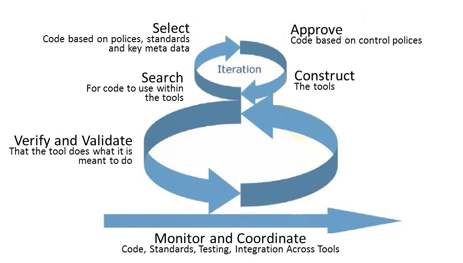
\includegraphics[width=5in]{Plan}
	\caption{High-Level Architecture}
	\label{fig-plan}
\end{figure}

Once at steady-state, each project will use 3-week (4 per quarter) sprints to develop and enhance their components. 
At the end of each sprint, integration across the feature sets will ensure coordination and compatibility.  
Experienced SLR authors and existing tool developers will have access to resulting sprint builds and have input into the product backlogs and priority assignments of these items (see attached support letters).  
Each team will construct a backlog of features that need to be developed for their specific feature set.
With the aid of the users of the specific features providing input, the project lead for each team will act as product owners to prioritize the backlog for each sprint.  
The graduate student will be responsible for high-level architecture and design decisions, including investigating various trade-offs in implementation choices.
The CAPS developers will implement and test the features in each sprint.
During the execution of the sprints and during the retrospectives at the end of the sprints we will identify cross-feature relationships and add them to the backlog for the appropriate feature sets.
The user communities for each of the feature sets will have the capability to be active testers to ensure features perform as expected.  

%The assignment of the feature sets will be based on needed expertise, current capabilities and programmatic learning objectives.  
%As an example of the programmatic learning objectives, CS students will be assigned to take the lead for core backplane tier features, while MIS students will take the lead for planning, coordination and monitoring features.  
%This assignment will draw on their experiences, coursework and career objectives.   
%Collectively the CS and MIS students will learn to work together and extend their professional comfort drawing upon the strengths of one another. 